\chapter{Data and methodologies}

\label{chapter:methodologies}

In this chapter, we describe the \ac{fmtod} data set in greater detail and
survey the performance of other studies that addressed this data set and its
tasks. Following this, we introduce the \ac{spp} model and describe the
methodologies used for answering our three research questions. Comprehensive
source code reflecting our methodologies can be found in our public GitHub
repository\footnote{\url{https://github.com/atreyasha/spp-explainability}}.

\section{Facebook Multilingual Task Oriented Dialog}

\citet{schuster-etal-2019-cross-lingual} originally released the \ac{fmtod} data
set to encourage research in cross-lingual transfer learning for
dialogue-oriented \ac{nlu} tasks; specifically from high-resource to
low-resource languages. The authors released the \ac{fmtod} data set with
English as the high-resource language providing $\sim$43k utterances, and
Spanish and Thai as low-resource languages providing a total of $\sim$14k
utterances. Furthermore, they streamlined the data set towards two key tasks;
namely intent classification and textual slot filling. In this thesis, we focus
solely on the English language intent classification task; which entails a
multi-label sequence classification task with a total of 12 classes from alarm,
reminder and weather-related domains. For brevity, we refer to the \ac{fmtod}
English language intent classification data set as the \ac{fmtod} data set.

We chose to work with the \ac{fmtod} data set since it is both a recently released
and well-studied data set
\citep{schuster-etal-2019-cross-lingual,zhang2019joint,zhang-etal-2020-intent}.
We focus on the English language intent classification task since it is a
relatively straightforward task which allows us to place a greater focus on
performance and explainability. Furthermore, the English language subset entails
the highest resources in the \ac{fmtod} data set. Finally, we find the \ac{fmtod} data
set's intent classification task especially attractive because it allows us
to test the \ac{spp} model on a multi-class \ac{nlu} problem; which is significantly
different from the focus on binary classification sentiment detection tasks in
\ac{sopa}. 

\subsection{Preprocessing}

Given that we are handling text-based data in the \ac{fmtod} data set, it is
necessary to preprocess this data first before proceeding with any modeling
steps. We enumerate our preprocessing steps below:

\begin{enumerate}{}
  \item We convert all \ac{fmtod} text samples into a lowercased format. This assists
  in simplifying and normalizing the textual data.
  \item Next, we remove data duplicates within the provided training, validation and test
  data partitions.
  \item Finally, we remove data duplicates which overlap between partitions.
  During this step, we do not remove any cross-partition duplicates from the
  test partition in order to keep it as similar as possible to the original test
  partition. This comes into importance later when we compare performance metrics
  on the test set with other studies.
\end{enumerate}

\begin{figure}[t!]
  \centering
  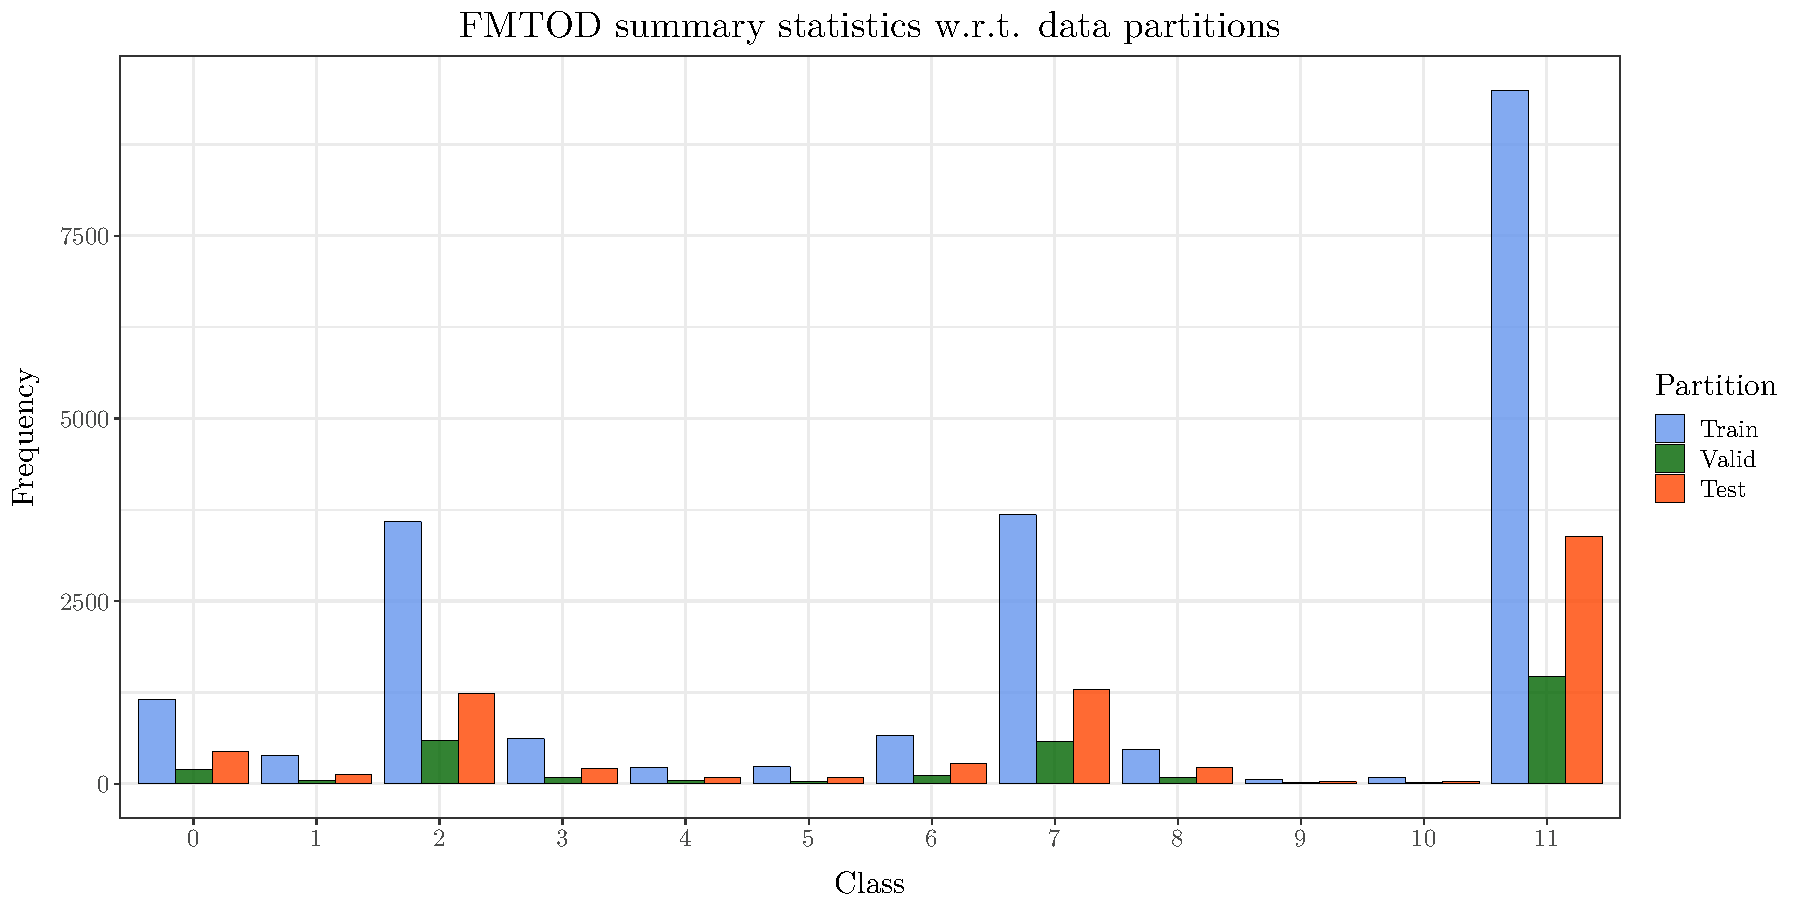
\includegraphics[width=14cm]{pdfs/generated/fmtod_summary_statistics.pdf}
  \caption{Frequency distribution of the preprocessed FMTOD data set classes grouped by
    partitions}
  \label{fig:fmtod}
\end{figure}

\begin{table}[t!]
  \centering
  \begin{tabular}{lllll}
    \toprule
    Class and description & Train & Validation & Test & $\Sigma$ \\
    \midrule
    0: \texttt{alarm/cancel\_alarm} & 1157 & 190 & 444 & 1791 \\
    1: \texttt{alarm/modify\_alarm} & 393 & 51 & 122 & 566 \\
    2: \texttt{alarm/set\_alarm} & 3584 & 596 & 1236 & 5416 \\
    3: \texttt{alarm/show\_alarms} & 619 & 83 & 212 & 914 \\
    4: \texttt{alarm/snooze\_alarm} & 228 & 49 & 89 & 366 \\
    5: \texttt{alarm/time\_left\_on\_alarm} & 233 & 30 & 81 & 344 \\
    6: \texttt{reminder/cancel\_reminder} & 662 & 114 & 284 & 1060 \\
    7: \texttt{reminder/set\_reminder} & 3681 & 581 & 1287 & 5549 \\
    8: \texttt{reminder/show\_reminders} & 474 & 82 & 217 & 773 \\
    9: \texttt{weather/check\_sunrise} & 63 & 13 & 25 & 101 \\
    10: \texttt{weather/check\_sunset} & 88 & 11 & 37 & 136 \\
    11: \texttt{weather/find} & 9490 & 1462 & 3386 & 14338 \\[5pt]
    \hline \hline \\[-10pt]
    $\Sigma$ & 20672 & 3262 & 7420 & 31354 \\
    \bottomrule
  \end{tabular}
  \caption{Frequencies of the preprocessed FMTOD data set classes grouped by
    partitions; $\Sigma$ signifies the aggregate sum statistic}
  \label{tab:fmtod}
\end{table}

During the preprocessing phase, many data duplicates were encountered and
correspondingly removed. Some of these duplicates observed were already present
in the original \ac{fmtod} data set, with additional duplicates being created from
the initial lowercasing step. After preprocessing, we obtain a lowercased
variant of the \ac{fmtod} data set with strictly unique data partitions. In the next
section, we describe the summary statistics of the preprocessed \ac{fmtod} data set.

\begin{table}[t!]
  \centering
  \begin{threeparttable}
    \begin{tabular}{lll}
      \toprule
      Class and description & Utterance length$^{\dagger}$ & Example$^{\ddagger}$ \\
      \midrule
      0: \texttt{alarm/cancel\_alarm} & 5.6 $\pm$ 1.9 & cancel weekly alarm \\
      1: \texttt{alarm/modify\_alarm} & 7.1 $\pm$ 2.5 & change alarm time \\
      2: \texttt{alarm/set\_alarm} & 7.5 $\pm$ 2.5 & please set the new alarm \\
      3: \texttt{alarm/show\_alarms} & 6.9 $\pm$ 2.2 & check my alarms. \\
      4: \texttt{alarm/snooze\_alarm} & 6.1 $\pm$ 2.1 & pause alarm please \\
      5: \texttt{alarm/time\_left\_on\_alarm} & 8.6 $\pm$ 2.1  & minutes left on my alarm \\
      6: \texttt{reminder/cancel\_reminder} & 6.6 $\pm$ 2.2 & clear all reminders. \\
      7: \texttt{reminder/set\_reminder} & 8.9 $\pm$ 2.5 & birthday reminders \\
      8: \texttt{reminder/show\_reminders} & 6.8 $\pm$ 2.2 & list all reminders \\
      9: \texttt{weather/check\_sunrise} & 6.7 $\pm$ 1.7 & when is sunrise \\
      10: \texttt{weather/check\_sunset} & 6.7 $\pm$ 1.7 & when is dusk \\
      11: \texttt{weather/find} & 7.8 $\pm$ 2.3 & jacket needed? \\[5pt]
      \hline \hline \\[-10pt]
      $\mu$ & 7.7 $\pm$ 2.5 & \textemdash \\
      \bottomrule
    \end{tabular}
    \begin{tablenotes}[flushleft]
      \footnotesize
      \item $^{\dagger}$Summary statistics follow the mean $\pm$
      standard-deviation format
      \item $^{\ddagger}$Short and simple examples were chosen for brevity and
      formatting purposes
    \end{tablenotes}
  \end{threeparttable}
  \caption{Utterance length summary statistics and examples for the preprocessed
    FMTOD data set; $\mu$ signifies the aggregate mean statistic}
  \label{tab:fmtod_examples}
\end{table}

\begin{table}[t!]
  \centering \def\arraystretch{1.3}
  \begin{tabular}{L{0.27\linewidth} L{0.45\linewidth} l}
    \toprule
    Study & Summary & Accuracy \\
    \midrule
    \citet{schuster-etal-2019-cross-lingual} & Bidirectional LSTM jointly trained on both the slot filling and intent classification tasks & 99.1$\%$ \\
    \citet{zhang2019joint} & BERT along with various decoders jointly fine-tuned on both the slot filling and intent classification tasks & 96.6--98.9$\%$ \\
    \citet{zhang-etal-2020-intent} & RoBERTa and XLM-RoBERTa fine-tuned on the English language and multilingual intent classification tasks along with WikiHow pre-training & 99.3--99.5$\%$ \\
    \bottomrule
  \end{tabular}
  \caption{Studies that addressed the FMTOD English language intent
    classification task along with their relevant summaries and accuracy
    ranges}
  \label{tab:fmtod_results}
\end{table}

\subsection{Summary statistics}

\label{section:fmtod_summary}

In regards to summary statistics of the preprocessed \ac{fmtod} data set, Figure
\ref{fig:fmtod} provides a visualization of the frequency distribution in the
data set grouped by classes and partitions; while Table \ref{tab:fmtod} shows
the same summary statistics in a tabular form with explicit frequencies. Based
on the summary statistics, we can observe that the preprocessed \ac{fmtod} data set
is significantly imbalanced with $\sim$45$\%$ of samples falling into Class 11
alone. We take this observation into consideration in later sections and apply
fixes to mitigate this data imbalance. In addition, we observe from Table
\ref{tab:fmtod_examples} that input utterances in the preprocessed \ac{fmtod} data
set are generally short; with a mean input utterance length of 7.7 and a
standard deviation of 2.5 tokens. Utterance length summary statistics were
computed with the assistance of the \ac{nltk} \texttt{Treebank} word tokenizer
\citep{bird-loper-2004-nltk}.

\subsection{Performance range}

\label{section:fmtod_performance}

Several recent studies have addressed the \ac{fmtod} English language intent
classification task using a variety of deep neural networks from bidirectional
\ac{lstm}s to large Transformer language models such as \ac{bert}
\citep{schuster-etal-2019-cross-lingual,zhang2019joint,zhang-etal-2020-intent}.
Table \ref{tab:fmtod_results} summarizes these studies along with their reported
accuracy scores on the \ac{fmtod} English language intent classification task.
Based on the presented results, we can observe that the competitive accuracy
range for the \ac{fmtod} English language intent classification task is
96.6-99.5$\%$.

\section{SoPa++}

Based on our analysis in Section \ref{section:sopa_post_hoc}, we found \ac{sopa}'s
explainability techniques to be localized and indirect. Furthermore, we believe
that these techniques did not fully capitalize on the rich theoretical
foundations offered by \ac{wfas} in the neural architecture; such as possible
extractions of \ac{nfas} and conversions to regular expressions. In order to
address these limitations, we introduce the main contribution of this thesis:
the \ac{spp} model. Etymologically, \ac{spp} derives its name from the variable
increment operator \texttt{"++"} used in programming languages such as C and
Java. In essence, the name \ac{spp} signifies an improvement or major modification
to the \ac{sopa} model. Some of the major modifications from \ac{sopa} to \ac{spp} include
the utility of strict linear-chain \ac{wfaws} over linear-chain \ac{wfas},
replacement of the \ac{mlp} in \ac{sopa} with quantized and transparent hidden layers
and the introduction of a new globalized and direct explanations by
simplification post-hoc explainability technique to simplify the black-box
\ac{spp} model into a transparent \ac{re} proxy model.

\subsection{Strict linear-chain WFA-$\omega$'s}

As mentioned in Section \ref{section:sopa}, \citet{schwartz2018sopa} constructed
the \ac{sopa} model with an ensemble of linear-chain \ac{wfas} which permitted both
$\epsilon$ and self-loop transitions. As noted in Section \ref{section:sopa_cg},
$\epsilon$ and self-loop transitions are useful constructs in abstracting \ac{wfas}
and allowing them to consume variable length strings. However, based on
experimentation during our development phase; we observed a key concern that the
highest scoring substrings in the linear-chain \ac{wfas} in \ac{sopa} tended to have a
large variation in string lengths due to the effect of both
$\epsilon$-transitions and self-loops. We believe that this reduced the impact
of \ac{sopa}'s explainability techniques due to a lack of consistency in the lengths
of highest scoring paths and substrings. As a result, the first change we decided
for was to remove both $\epsilon$ and self-loop transitions in constituent \ac{wfas}
or patterns. With this change, we could at least ensure that each \ac{wfa} would
always consume strings of fixed lengths.

However, consuming strings of fixed lengths could also be seen as a form of
overfitting in the model; since a model could simply memorize short strings or
phrases and would not necessarily incorporate any form of generalization. To
address this concern, we include a wildcard transition which we define here as a
$\omega$-transition. Allowing for such a transition was only natural since
wildcards are already crucial parts of regular expressions; which as we
mentioned are equivalent to \ac{fas}. To provide formalisms for this modification, we
provide the following definition for a \ac{wfaw}.

\begin{definition}[Weighted finite-state automaton-$\omega$]
  \label{def:wfa_w}
  A weighted finite-state automaton-$\omega$ over a semiring $\mathbb{K}$ is a
  5-tuple $\mathcal{A} = \langle \Sigma, \mathcal{Q}, \bm{\Gamma}, \bm{\lambda}, \bm{\rho}
  \rangle$, with:

  \begin{itemize}
  \itemsep0em
    \item[--] a finite input alphabet $\Sigma$;
    \item[--] a finite state set $\mathcal{Q}$;
    \item[--] transition matrix $\bm{\Gamma}: \mathcal{Q} \times \mathcal{Q} \times (\Sigma \cup \{\omega\}) \rightarrow \mathbb{K}$;
    \item[--] initial vector $\bm{\lambda}: \mathcal{Q} \rightarrow \mathbb{K}$;
    \item[--] and final vector $\bm{\rho}: \mathcal{Q} \rightarrow \mathbb{K}$.
  \end{itemize}

  \begin{remark}
    An $\omega$ transition is equivalent to a wildcard transition, which
    consumes an arbitrary token input and moves to the next state.
  \end{remark}

  \begin{remark}
    Besides the inclusion of the $\omega$-transition and removal of the
    $\epsilon$-transition, a \ac{wfaw} has all of the same characteristics
    as the \ac{wfa} defined in Definition \ref{def:wfa}.
  \end{remark}
\end{definition}

Comparing with the linear-chain \ac{wfas} used in \citet{schwartz2018sopa} as per
Section \ref{section:sopa_lc_wfa}, our \textit{strict} linear-chain \ac{wfaw}
is similarly allotted a sequence of $|\mathcal{Q}|$ states. However, each state
$i$ in the linear-chain \ac{wfaw} only has two possible outgoing transitions;
namely a \textbf{$\bm{\omega}$-transition} which consumes an arbitrary input
token and transitions to state $i+1$ and a \textbf{main-path transition} which
consumes a specific token and transitions to state $i+1$. Because of the
elimination of self-loop transitions, we refer to our linear-chain \ac{wfaw}
as strict linear-chain \ac{wfaw} as per Remark
\ref{rmk:strict_linear_chain}. Similar to \citet{schwartz2018sopa}, we utilize
only the max-sum and max-product semirings in our strict linear-chain
\ac{wfaws}.

\begin{figure}[t!]
  \centering
  \includegraphics[width=14cm]{pdfs/generated/w_nfa_linear_chain/main.pdf}
  \caption{Strict linear-chain NFA with
    $\omega$ (blue) and main-path (black) transitions}
  \label{fig:omega_fa}
\end{figure}

Next, we provide a mathematical formulation of the modified transition matrix
$\bm{\Gamma}$ in our strict linear-chain \ac{wfaw}. Here, $\bm{\Gamma}(x)$ represents a
$|Q|\times|Q|$ matrix containing transition scores when consuming an input token
$x$. $[\bm{\Gamma}(x)]_{i,j}$ corresponds to the cell value in $\bm{\Gamma}(x)$ for row
$i$ and column $j$ and represents the transition score when consuming token $x$
and transitioning from state $i$ to $j$.

\begin{equation}
  \label{eq:spp_transition_matrix_main}
  [\bm{\Gamma}(x)]_{i,j} =
  \begin{cases}
    \bm{w}_i \cdot \bm{v}_x + b_i  & \text{if } j = i + 1 \text{ (main-path transition),} \\
    \bar{0} & \text{otherwise.}
  \end{cases}
\end{equation}

Here, $\bm{w}_i$ and $b_i$ are learnable vectors and scalar biases
parameterizing transitions out of state $i$ to state $i+1$. $\bm{v}_x$
represents the word embedding for token $x$ and $\bar{0}$ represents the zero
value in the semiring used as per Definition \ref{def:semiring}. Similarly,
$\omega$-transitions are parameterized with the following representation in
$\bm{\Gamma}$:

\begin{equation}
  \label{eq:spp_transition_matrix_omega}
  [\bm{\Gamma}(\omega)]_{i,j} =
  \begin{cases}
    c_i  & \text{if } j = i + 1 \text{ ($\omega$-transition)} \\
    \bar{0} & \text{otherwise.}
  \end{cases}
\end{equation}

Here, $c_i$ represents a learnable scalar bias for $\omega$-transitions out of
state $i$ to state $i+1$. Finally as per \citet{schwartz2018sopa}, we fix the
initial vector $\bm{\lambda} = [\bar{1}, \bar{0}, \ldots, \bar{0}]$ and the final
vector $\bm{\rho} = [\bar{0}, \bar{0}, \ldots, \bar{1}]$, where $\bar{1}$ and
$\bar{0}$ represent the one and zero values specified in the semiring as per
Definition \ref{def:semiring}. The time-complexity of the Viterbi algorithm to
compute the string score for our linear-chain \ac{wfaws} is
$O(|Q||\bm{x}|)$, where $|\mathcal{Q}|$ refers to the number of states and
$|\bm{x}|$ refers to the length of the input string.

Ultimately, the introduction of a strict linear-chain \ac{wfaw} allows us to
attain fixed string length consumption with an added layer of generalization
because of the introduction of wildcards. An example of a strict linear-chain
\ac{nfa} extracted from a strict linear-chain \ac{wfaw} is shown in Figure
\ref{fig:omega_fa}. Interestingly, we can observe that this \ac{nfa} corresponds to
the Perl-compatible regular expression \texttt{``what a (great|entertaining)
  [\^{}\textbackslash s]+ !''}, where
\texttt{[\^{}\textbackslash s]+} refers to any set of consecutive
characters which are not separated by a space character. We can therefore infer
that a $\omega$-transition in a \ac{fa} corresponds to the
\texttt{[\^{}\textbackslash s]+} regular expression term.

\begin{algorithm}[t!]
  \small
  \caption{Strict linear-chain WFA-$\omega$ document score$^*$}
  \label{algo:lc_wfa_w_document_score}
  \begin{algorithmic}[1]
    \Require{Strict linear-chain \ac{wfaw} (denoted as $\mathcal{A}$) and document $\bm{y}$}
    \Ensure{Document score $s_{\text{doc}}(\bm{y})$}
    \Statex
    \Function{docscore}{$\mathcal{A}, \bm{y}$}
    \State $\bm{h}_0 \gets \big[\bar{1}, -\infty, \ldots, -\infty\big]$ \Comment{Create
      initial hidden state vector $\bm{h}_0: \mathcal{Q} \rightarrow \mathbb{K}$}
    \For{$i \gets 1,2,\ldots,\bm{|y|}$} \Comment{Sequentially iterate over each
      token $y_i \in \bm{y}$}
    \State $\bm{m} \gets \big[[\bm{\Gamma}(y_i)]_{1,2}, [\bm{\Gamma}(y_i)]_{2,3}, \ldots,
    [\bm{\Gamma}(y_i)]_{|\mathcal{Q}|-1,|\mathcal{Q}|}\big]$ \Comment{Main-path scores for token $y_i$}
    \State $\bm{\omega} \gets \big[[\bm{\Gamma}(\omega)]_{1,2}, [\bm{\Gamma}(\omega)]_{2,3}, \ldots,
    [\bm{\Gamma}(\omega)]_{|\mathcal{Q}|-1,|\mathcal{Q}|}\big]$
    \Comment{State-wise wildcard scores}
    \State $\bm{m'} \gets \bm{m} \otimes \bm{h}_{i-1}[:-1]$ \Comment{Path
      score with main-path transitions$^{\dagger}$}
    \State $\bm{\omega'} \gets \bm{\omega} \otimes \bm{h}_{i-1}[:-1]$ \Comment{Path
    score with $\omega$ transitions$^{\dagger}$}
    \State $\bm{h}_{i} \gets [\bar{1}] \mathbin\Vert \max(\bm{m'}, \bm{w'})$
    \Comment{Concatenate $\bar{1}$ to maximum of $\bm{m'}$ and $\bm{\omega'}$}    
    \EndFor
    \State $s_{\text{doc}}(\bm{y}) \gets  \max_{i \in 1,2,...,|\bm{y}|}
    \bm{h}_{i}[-1]$
    \Comment{Get maximum of hidden vector final states$^{\ddagger}$}
    \State \Return $s_{\text{doc}}(\bm{y})$
    \EndFunction
  \end{algorithmic}
  \algcomment{
    $^*$$\otimes$ and $\bar{1}$ are
    derived from max-based semirings with all semiring operations being element-wise \\
    $^{\dagger}\bm{h}_{i}[:-1]$ follows the Python indexing syntax
    and implies keeping all elements of $\bm{h}_{i}$ except the last \\
    $^{\ddagger}\bm{h}_{i}[-1]$ follows the Python indexing syntax and implies
    retrieving the last element of the vector $\bm{h}_{i}$
  }
\end{algorithm}

\subsection{Document score}

Similar to \citet{schwartz2018sopa}, \ac{spp} was intended to compute scores for
entire documents and not just fixed-length strings using the strict linear-chain
\ac{wfaw}. To achieve this, we propose Algorithm
\ref{algo:lc_wfa_w_document_score} to compute the document score
$s_{\text{doc}}(\bm{y})$ for an arbitrary document $\bm{y}$. Here, we score all
consecutive substrings in a document $\bm{y}$ using either the max-sum or
max-product semirings assisted with the Viterbi algorithm. Following from this,
the document score $s_{\text{doc}}(\bm{y})$ would reflect the highest path score
corresponding to a substring in an arbitrary document $\bm{y}$.

\subsection{TauSTE}

In Section \ref{section:ste}, we described the concept of a \ac{ste} in
quantized neural networks and explained how \ac{ste}s function in both their
forward and backward passes. Furthermore, we provided a motivation as to why
\ac{ste}s and other quantized activation functions are of interest; for example
in low-precision computing. In \ac{spp}, we make use of a variant of the
\ac{ste} activation function which we define here as the \ac{tauste}.

\begin{equation}
  \label{eq:tau_ste_forward}
  \text{TauSTE}(x)=
  \begin{cases}
    1 & x \in (\tau, +\infty) \\
    0 & x \in (-\infty, \tau]
  \end{cases}
\end{equation}

\begin{equation}
  \label{eq:tau_ste_backward}
  \text{TauSTE}'(x)=
  \begin{cases}
    1 & x \in  (1, +\infty) \\
    x & x \in [-1, 1] \\
    -1 & x \in (-\infty, -1) \\
  \end{cases}
\end{equation}

\begin{figure}[t!]
  \centering
  \includegraphics[width=14cm]{pdfs/generated/tau_ste_applied/main.pdf}
  \caption{TauSTE's forward and backward passes}
  \label{fig:tau_ste}
\end{figure}

A visualization of the \ac{tauste}'s forward and backward passes is shown in Figure
\ref{fig:tau_ste}. As we can see, there are two key changes from the vanilla \ac{ste}
to the \ac{tauste}. Firstly, the threshold for activation in the forward function is
now governed by a $\tau$-threshold such that $\tau \in \mathbb{R}$. This was
done to allow for some degree of freedom in deciding the activation threshold.
Secondly, the backward pass returns the identity function on $x \in [-1,1]$ and
remains fixed at -1 or +1 beyond these limits. This restriction was placed to
ensure that gradients do not blow up in size.

We chose to use the \ac{tauste} because we believed it could prove useful for
the explainability purposes of our \ac{spp} model. This is because the
\ac{tauste} activation function simplifies continuous inputs into discrete
outputs; thereby reducing the information content of the signal it receives. In
later sections, we show how we capitalize on this reduction in signal
information in our \ac{spp} model for our explanations by simplification
post-hoc explainability technique.

\subsection{Computational graph}

With the core modifications in the \ac{spp} model explained, we now shift to
describing the computational graph of the \ac{spp} model by
referring to its various neural components. This description is linked to the
visualization of the computational graph of \ac{spp} in Figure \ref{fig:spp_cg}.
Firstly, we utilize \ac{nltk}'s default \texttt{Treebank} word tokenizer
\citep{bird-loper-2004-nltk} to conduct tokenization of input utterances into
word-level tokens. Next, we pad input utterances with special \texttt{[START]}
and \texttt{[END]} tokens at the start and end indices of the utterances to
signify locations where the utterance begins and ends. Finally, we utilize
\ac{glove} 6B 300-dimensional uncased word-level embeddings
\citep{pennington2014glove} to project the input tokens to continuous numerical
spaces. 

\begin{figure}[t!]
  \centering
  \includegraphics[width=15cm]{pdfs/generated/spp_computational_graph/main.pdf}
  \caption{SoPa++ computational graph; flow of graph is
    from bottom to top and left to right }
  \label{fig:spp_cg}
\end{figure}

Following this, we use our ensemble of $m \in \mathbb{N}$ strict linear-chain
\ac{wfaws} to traverse the input utterance and provide individual document
scores for this utterance; as prescribed by Algorithm
\ref{algo:lc_wfa_w_document_score}. When processing each input token, we monitor
the final states of each of the $m$ strict linear-chain \ac{wfaws} and
max-pool the score present in this state. In the edge case that an input string
was too short for the final state of a \ac{wfaw} to register a non-$\bar{0}$
score, we simply discard this score in further analysis. This description so far
corresponds to the lower half of Figure \ref{fig:spp_cg}. After max-pooling
scores from all the $m$ strict linear-chain \ac{wfaws}, we then pass this
collection of pattern scores for further processing using \ac{spp}'s hidden neural
components; which can be seen in the upper portion of Figure \ref{fig:spp_cg}.
Firstly, we apply layer normalization \citep{ba2016layer} to all pattern scores
without any additional affine transformations. We omit the affine transformation
to not alter any of the pattern score information content and use layer
normalization as an expedient means of projecting the values of pattern scores
to a standard normal distribution. This normalization process guarantees that
pattern scores would be small in size and have a roughly even distribution of
positive and negative values around 0.

Layer normalization becomes very useful as we correspondingly encounter the
\ac{tauste} layer. Here, the \ac{tauste} layer maps all inputs which are strictly larger
than the $\tau \in \mathbb{R}$ threshold to 1 and all others inputs to zero.
Naturally, the \ac{tauste} layer is only useful when it is able to discriminate the
inputs by mapping some of them to 1 and some to 0, instead of always mapping all
inputs to either 1 or 0. Without layer normalization, the \ac{tauste} layer would not
be able to perform its function since pattern scores tend to be mostly positive
with differing ranges. Layer normalization therefore helps to project these
variations of pattern scores to a uniform range; which ultimately allows the \ac{tauste}
layer to discriminate inputs and produce diverse binary outputs.

A natural criticism of the \ac{tauste} layer could be that it strongly limits
the flow of information in the \ac{spp} model. While the binarization present in
this layer does indeed limit the rich flow of continuous numerical information,
it is still worth noting that this layer can preserve significant information
given a sufficiently large $m$ value, corresponding to the number of strict
linear-chain \ac{wfaw} and \ac{tauste} neurons. For example, if we allow for
$m=40$ and therefore provide 40 \ac{wfaw} and \ac{tauste} neurons, we can have a
total of 2$^{40}\approx1.1\times10^{12}$ binary state possibilities; which is
slightly greater than one trillion possible binary states. To provide some
context to this order of magnitude, the aforementioned number of possibilities
is roughly equal to estimated number of stars present in the Andromeda Galaxy
\citep{10.1093/mnras/stu879}. This would imply that despite the reduction in
information content in the \ac{tauste} layer, there are still sufficient
mappable states available to learn various representations relevant to output
classes; given a large enough $m$ value or number of \ac{wfaw}.

After binarizing the hidden values in the \ac{tauste} layer, we apply a simple linear
transformation to the \ac{tauste} binary outputs to modify their dimensionality from
$m$ to $n \in \mathbb{N}$, where the $n$ represents the number of output
classes. We specifically chose a linear transformation layer over a \ac{mlp} because
linear regressors are known to be transparent models
\citep{arrieta2020explainable} and this is a feature which ultimately assists us
in our explanations by simplification post-hoc explainability technique, which
we describe in greater detail in the next sections. Finally, we apply a softmax
function over the linear outputs to project them to probabilistic spaces and
then compute an argmax to extract the highest scoring index which represents the
predicted class. In the case of Figure \ref{fig:spp_cg}, the output class for
the input preprocessed utterance \texttt{``[START] 10 day weather forecast
  [END]''} is the \texttt{weather/find} class which corresponds to class index 11.

\subsection{Transparency}

\label{section:spp_transparency}

In regards to transparency, \ac{spp} is a hybridized model consisting of \ac{rnn},
\ac{cnn} and weighted finite-state neural components similar to that of \ac{sopa}.
Following the arguments of \citet{arrieta2020explainable} related to the
black-box natures of \ac{rnn}s and \ac{cnn}s, we can conclude that \ac{spp} would
correspondingly fall into the black-box model category. Because of this
classification, the \ac{spp} model would require post-hoc explainability
techniques in order to explain its inner mechanisms. We capitalize on the rich
theoretical foundations offered by the constituent \ac{wfas} in \ac{spp} and
propose a new globalized and direct explanations by simplification post-hoc
explainability technique to simplify the black-box \ac{spp} model into a
transparent \ac{re} proxy model.

\section{RE proxy}

In this section, we describe the key processes required to convert a fully
trained black-box \ac{spp} model into a transparent \ac{re} proxy model. We start
off with the introduction of a path-augmented document scoring algorithm and the
extraction of the \ac{re} lookup layer. Following this, we describe the assembly
and computational graph of the \ac{re} proxy model. Finally, we provide some
comments on explainability-related aspects of the simplified \ac{re} proxy model
and its antecedent \ac{spp} counterpart.

\subsection{Path-augmented document score}

\begin{algorithm}[t!]
  \small
  \caption{Strict linear-chain WFA-$\omega$ path-augmented document score$^*$}
  \label{algo:lc_wfa_w_document_score_trace}
  \begin{algorithmic}[1]
    \Require{Strict linear-chain \ac{wfaw} (denoted as $\mathcal{A}$) and document $\bm{y}$}
    \Ensure{Document score $s_{\text{doc}}(\bm{y})$ and its corresponding path $\pi_{\text{doc}}(\bm{y})$}
    \Statex
    \Function{docscore\_path}{$\mathcal{A}, \bm{y}$}
    \State $\bm{h}_0 \gets \big[\bar{1}, -\infty, \ldots, -\infty\big]$ \Comment{Create
      initial hidden state vector $\bm{h}_0: \mathcal{Q} \rightarrow \mathbb{K}$}
    \For{$i \gets 1,2,\ldots,\bm{|y|}$} \Comment{Sequentially iterate over each
      token $y_i \in \bm{y}$}
    \State $\bm{m} \gets \big[[\bm{\Gamma}(y_i)]_{1,2}, [\bm{\Gamma}(y_i)]_{2,3}, \ldots,
    [\bm{\Gamma}(y_i)]_{|\mathcal{Q}|-1,|\mathcal{Q}|}\big]$ \Comment{Main-path scores for token $y_i$}
    \State $\bm{\omega} \gets \big[[\bm{\Gamma}(\omega)]_{1,2}, [\bm{\Gamma}(\omega)]_{2,3}, \ldots,
    [\bm{\Gamma}(\omega)]_{|\mathcal{Q}|-1,|\mathcal{Q}|}\big]$
    \Comment{State-wise wildcard scores}
    \State $\bm{m'} \gets \bm{m} \otimes \bm{h}_{i-1}[:-1]$ \Comment{Path
      score with main-path transitions$^{\dagger}$}
    \State $\bm{\omega'} \gets \bm{\omega} \otimes \bm{h}_{i-1}[:-1]$ \Comment{Path
    score with $\omega$ transitions$^{\dagger}$}
    \State $\bm{h}_{i} \gets [\bar{1}] \mathbin\Vert \max(\bm{m'}, \bm{w'})$
    \Comment{Concatenate $\bar{1}$ to maximum of $\bm{m'}$ and $\bm{\omega'}$}
    \State $\pi_i \gets \text{trace}(h_i[-1])$
    \Comment{Back-trace path $\pi_i$ corresponding to $h_i[-1]^{\ddagger}$}
    \EndFor
    \State $j \gets \argmax_{i \in 1,2,...,|\bm{y}|}
    \bm{h}_{i}[-1]$
    \Comment{Get index of final states' maximum$^{\ddagger}$}
    \State $s_{\text{doc}}(\bm{y}) \gets \bm{h}_{j}[-1]$
    \Comment{Get maximum final state value$^{\ddagger}$}
    \State $\pi_{\text{doc}}(\bm{y}) \gets \pi_j$
    \Comment{Get path of maximum final state value}
    \State \Return $[s_{\text{doc}}(\bm{y}), \pi_{\text{doc}}(\bm{y})]$
    \EndFunction
  \end{algorithmic}
  \algcomment{
    $^*$$\otimes$ and $\bar{1}$ are
    derived from max-based semirings with all semiring operations being element-wise \\
    $^{\dagger}\bm{h}_{i}[:-1]$ follows the Python indexing syntax
    and implies keeping all elements of $\bm{h}_{i}$ except the last \\
    $^{\ddagger}\bm{h}_{i}[-1]$ follows the Python indexing syntax and implies
    retrieving the last element of the vector $\bm{h}_{i}$
  }
\end{algorithm}

One major advantage of the Viterbi algorithm, as per Definition
\ref{def:string_score}, is its ability to return the highest path score which
can ultimately allow for attribution to a certain path and substring in a
document. In order to simplify \ac{spp} into a \ac{re} proxy model, we first
need to modify our document scoring algorithm to not only return the document
score $s_{\text{doc}}(\bm{y})$ but also its corresponding path
$\pi_{\text{doc}}(\bm{y})$. This process is described as a path-augmented
document score in Algorithm \ref{algo:lc_wfa_w_document_score_trace}, where we
trace the exact path of each transition and return the best path in addition to
the highest path score. Similar to Algorithm \ref{algo:lc_wfa_w_document_score},
this algorithm has a time-complexity of $O(|Q||\bm{x}|)$, where $|\mathcal{Q}|$
refers to the number of states in a strict linear-chain \ac{wfaw} and $|\bm{x}|$
refers to the length of the input string. It is also worth mentioning that the
highest scoring path returned ultimately reflects a set of transitions in the
form of a strict linear-chain \ac{nfa}; which can correspondingly be transformed
into a regular expression. Therefore, it can be inferred that Algorithm
\ref{algo:lc_wfa_w_document_score_trace} returns the best scoring regular
expression corresponding to the document score from a certain strict
linear-chain \ac{wfaw}.

\subsection{RE lookup layer}

The next step in simplifying a fully-trained \ac{spp} to a \ac{re} proxy model is the
extraction of a \ac{re} lookup layer. To motivate this process, we shortly revert to
the \ac{spp} computational graph in Figure \ref{fig:spp_cg}. The \ac{tauste} layer
filters input signals from normalized pattern scores and provides +1 outputs for
normalized pattern scores which exceed the $\tau$-threshold. Since pattern
scores correspond to document scores and document scores can be augmented with
best paths and regular expressions as per Algorithm
\ref{algo:lc_wfa_w_document_score_trace}, we can assign the activation of each
\ac{tauste} neuron for each input utterance with an "activating" regular expression.
By iterating over all our training data, we can collect many such "activating"
regular expressions which activate the various \ac{tauste} neurons; such that each
\ac{tauste} neuron $\textbf{N}_i$ is assigned a set of "activating" regular expressions
\textbf{\{RE\}$_i$}. The collection of all regular expressions
$[\{\textbf{RE}\}_1, \ldots, \{\textbf{RE}\}_m]$ which activate $m$ \ac{tauste}
neurons is known as the \ac{re} lookup layer. Overall, the \ac{re} lookup layer represents
a knowledge base of important regular expressions that cause the \ac{spp} model to
make weighted decisions. This process of extracting the \ac{re} lookup layer from
the \ac{spp} model is reflected in Algorithm \ref{algo:simplification_process}.

\begin{algorithm}[t!]
  \small
  \caption{Extracting RE lookup layer from SoPa++}
  \label{algo:simplification_process}
  \begin{algorithmic}[1]
    \Require{Trained SoPa++ model $\mathcal{S}$ and training data $[\bm{y}_1, \ldots, \bm{y}_t]$}
    \Ensure{RE lookup layer $[\{\textbf{RE}\}_1, \ldots, \{\textbf{RE}\}_m]$}
    \Statex
    \Function{extract\_lookup}{$\mathcal{S}, [\bm{y}_1, \ldots, \bm{y}_t]$}
    \State $[\{\textbf{RE}\}_1, \ldots, \{\textbf{RE}\}_m] \gets [\emptyset,
    \ldots, \emptyset]$
    \Comment{Initialize RE lookup layer}
    \For{$i \gets 1,2,\ldots,t$}
    \Comment{Loop over training data}
    \For{$j \gets 1,2,\ldots,m$}
    \Comment{Loop over \ac{wfaws} in $\mathcal{S}$}
    \State $\mathcal{A}_j \gets \text{get\_WFA}(\mathcal{S}, j)$
    \Comment{Get \ac{wfaw} by index}
    \State $s^j_{\text{doc}}(\bm{y}_i), \pi^j_{\text{doc}}(\bm{y}_i) \gets
    {\small\textsc{docscore\_path}}(\mathcal{A}_j, \bm{y}_i)$
    \Comment{As per Algorithm \ref{algo:lc_wfa_w_document_score_trace}}
    \If{TauSTE$(s^j_{\text{doc}}(\bm{y}_i)) == 1$}
    \State $\{\textbf{RE}\}_j \gets \{\textbf{RE}\}_j \cup
    \pi^j_{\text{doc}}(\bm{y}_i)$
    \Comment{Save $\pi^j_{\text{doc}}(\bm{y}_i)$ if it activates TauSTE} 
    \EndIf
    \EndFor
    \EndFor
    \State \Return $\text{compress}([\{\textbf{RE}\}_1, \ldots, \{\textbf{RE}\}_m])$
    \Comment{Compress RE lookup layer} 
    \EndFunction
  \end{algorithmic}
\end{algorithm}

This leads us to several interesting conclusions. Firstly, we observe here that
the \ac{tauste} layer is not only useful for reducing information complexity; but
also for attributing causal links in \ac{spp}'s decision-making. In this case,
the causal links are the "activating" regular expressions returned by the
strict linear-chain \ac{wfaw} when computing the path-augmented document
score. Next, we can also observe the effect of the $\tau$-threshold on the \ac{re}
lookup layer. If the $\tau$-threshold is low, we effectively allow more \ac{tauste}
neurons to be activated and therefore allow more regular expressions from the
strict linear-chain \ac{wfaw} to be saved in the \ac{re} lookup layer.
Contrastingly, if the $\tau$-threshold is high; we allow fewer \ac{tauste} neurons to
be activated and therefore allow fewer regular expressions to be saved in the \ac{re}
lookup layer. It is not necessarily clear whether small or large
$\tau$-thresholds are better for performance; but a larger $\tau$-threshold and
therefore smaller \ac{re} lookup layer could be beneficial for explainability
purposes since the \ac{re} knowledge base would be smaller and possibly easier
to comprehend for a human. 

\begin{figure}[t!]
  \centering
  \includegraphics[width=15cm]{pdfs/generated/regex_computational_graph/main.pdf}
  \caption{RE proxy computational graph; flow of graph is
    from bottom to top and left to right}
  \label{fig:regex_cg}
\end{figure}

\subsection{Assembling RE proxy}

The final step in simplifying a fully-trained \ac{spp} model into a \ac{re}
proxy model is to assemble the \ac{re} proxy model using the \ac{re} lookup and
\ac{spp} linear layers. Specifically, for a given \ac{spp} model; we firstly
extract the \ac{re} lookup layer. Then, we combine the \ac{re} lookup layer and
the \ac{spp} linear layer in order to create the \ac{re} proxy model. A
visualization of this is shown in Figure \ref{fig:regex_cg} and we can observe
how the \ac{re} lookup layer essentially replaces most of the lower neural
components of the \ac{spp} model up until the \ac{tauste} layer. The resulting
\ac{re} proxy sen this process of assembly, it is important to note that each \ac{spp} model
allows for exactly one \ac{re} proxy model to be assembled. Therefore, \ac{spp}
and \ac{re} proxy models occur in model pairs.

One major limitation of the \ac{re} proxy model is in its \ac{re} lookup layer.
Since the \ac{re} lookup layer is essentially a memorized knowledge base, it
could contribute to overfitting on the training data and result in a \ac{re}
proxy model that is not representative of the \ac{spp} model on unseen data.
While this limitation could theoretically be offset by the presence of
sufficient variable-length regular expressions with wildcards in the \ac{re}
lookup layer, it would ultimately boil down to an empirical investigation to
quantify how similarly the \ac{re} proxy model performs compared to its
antecedent \ac{spp} model on previously unseen data.

\subsection{Computational graph}

\label{section:re_cg}

We now provide a description of the computational graph of the assembled \ac{re}
proxy model with reference to Figure \ref{fig:regex_cg}. Similar to the
computational graph of \ac{spp}, we process our input text sequentially.
However, instead of using token embeddings and neural network components; we
pass our input utterance through our \ac{re} lookup layer which conducts
substring matches over all sets of regular expressions. If any regular
expression in the set $\{\textbf{RE}\}_i$ matches the input utterance, the index of
this \ac{re} set if given a value of 1. If no regular expression in the set
matches, the index of this \ac{re} set is given a value of 0. These values are
assembled into a binary vector that mimics the outputs of the \ac{tauste} layer
in the antecedent \ac{spp} model. This binary vector is then passed to the
linear layer; which transforms the binary vector back into continuous space with
the appropriate dimensionality. Following softmax and argmax operations, we
arrive at our predicted output class. It is worth mentioning that while the
execution of the \ac{spp} forward pass can be accelerated due to tensor-based
parallelization with hardware acceleration on a \ac{gpu}, the forward pass of
the \ac{re} proxy model is significantly slower since we utilized an unoptimized
single-threaded lookup process to match regular expressions in the \ac{re}
lookup layer.

\subsection{Transparency}

\label{section:re_transparency}

So far, we have described the process of simplifying a fully-trained black-box
\ac{spp} model into a \ac{re} proxy model. We now investigate the \ac{re} proxy model and
comment on its degree of transparency. In essence, a \ac{re} proxy model consists of
a \ac{re} lookup layer followed by a linear regressor. The \ac{re} lookup layer can be
seen as a rules-based learner component where inputs are processed via clear and
interpretable \ac{re} matching rules to produce outputs. Since both rules-based
learners and linear regressors can be considered as transparent models as per
\citet[Page 7, Section 3]{arrieta2020explainable}, we could theoretically
classify the \ac{re} proxy model as a transparent model. However, it is important to
note that this is only a theoretical argument which could be disproven in given
practical cases. For example as per \citet[Page 9, Table
2]{arrieta2020explainable}, rules-based learners and linear regressors could be
viewed as black-box models if they require the handling of an incomprehensible
number of rules or input features. This could also be the case for the \ac{re} proxy
model depending most importantly on the size of the \ac{re} lookup layer.

\subsection{Explainability}

We now provide additional comments on the explanations by simplification
post-hoc explainability technique to simplify a fully-trained black-box \ac{spp}
model into a transparent \ac{re} proxy model. Firstly, we would assign the target
audience of this explainability technique as expert end-users compared to the
inferred target audience of average end-users for the \ac{sopa} model. We designate
expert end-users as our target audience mainly because the process of constructing
and understanding the \ac{re} proxy model is not as straightforward as the local
explanations and feature relevance techniques in \ac{sopa} as per Section
\ref{section:sopa_post_hoc}.

Next, we evaluate the quality of the explanations by simplification post-hoc
explainability technique using the three guidelines detailed in Section
\ref{section:xai_metrics}. Regarding the constrictive quality, it is likely that
the \ac{re} proxy model meets this criterion since the linear layer contains
easily interpretable weights which are assigned to matched regular expressions;
thereby providing additive numerical evidence as to why one feature was more
important than another. Regarding causal links, it is likely that the \ac{re}
proxy model meets this criterion since the \ac{re} lookup layer matches fixed
regular expressions whose binary matching scores are then clearly propagated
from the start to the end of the model. Therefore, a decision occurring at the
end of the model could be causally attributed to features at the start of the
model. Regarding the selective quality, it is likely that the \ac{re} proxy
model meets this criterion since the linear weights applied to matched regular
expressions can be easily ranked to understand which were the most important
causal links influencing the model's decision.

Overall, we gather three key observations regarding the explanations by
simplification technique of the \ac{spp} model. Firstly, we find that this
technique is globalized compared to the localized methods of \ac{sopa}; since it
results in the production of a globally synthesized \ac{re} proxy model. Next,
we find that this technique is direct since it conveys end-to-end causal links
and does not use indirect feature relevance explainability techniques as in
\ac{sopa}. Finally, we observe that this technique likely fulfills all three
guidelines for good explanations; compared to \ac{sopa} fulfilling two of these
guidelines.

\begin{table}[t!]
  \centering \def\arraystretch{1.3}
  \begin{tabular}{L{0.275\linewidth} L{0.3\linewidth} L{0.3\linewidth}}
    \toprule
    Characteristic & SoPa & SoPa++ \\
    \midrule
    Text casing & True-cased & Lower-cased \\ 
    Token embeddings & GloVe 840B 300-dimensions & GloVe 6B 300-dimensions \\
    \ac{wfas} & Linear-chain \ac{wfas} with $\epsilon$, self-loop and main-path transitions & Strict linear-chain \ac{wfaws} with $\omega$ and main-path transitions \\
    Hidden layers & Multi-layer perceptron after max-pooling & Layer normalization, \ac{tauste} and linear transformation after max-pooling \\
    Post-hoc explainability technique(s) & Local explanations, feature relevance & Explanations by simplification \\
    \bottomrule
  \end{tabular}
  \caption{Summarized differences for SoPa vs. SoPa++}
  \label{tab:sopa_spp_comparison}
\end{table}

\section{Differences between SoPa and SoPa++}

To wrap up this current segment on the \ac{spp} model, we summarize the key
differences between \ac{sopa} and \ac{spp} as shown in Table
\ref{tab:sopa_spp_comparison}. The most significant changes in \ac{spp} include
the modification of linear-chain \ac{wfas} to strict linear-chain \ac{wfaws},
the replacement of the \ac{mlp} with layer normalization, \ac{tauste} and linear
layers and the introduction of the explanations by simplification post-hoc
explainability technique to create \ac{re} proxy models. With the construction
of \ac{spp} and its \ac{re} proxy models established, we now proceed to describe
the methodologies used to answer our three research questions.

\section{RQ1: Evaluating performance of SoPa++}

In this section, we describe the methodologies used to answer our first research
question regarding competitive performance of the \ac{spp} model on the
\ac{fmtod} data set. Specifically, we describe how we train the \ac{spp} model
and afterwards, how we evaluate and compare its performance to other studies.

\subsection{Training}

\label{section:spp_training}

First and foremost, we address the issue of data imbalance in the \ac{fmtod}
data set as mentioned in Section \ref{section:fmtod_summary}. For this, we chose
a simple but effective solution of upsampling all minority data classes such
that they would have the same frequency as the majority class. We chose this
approach over other approaches such as gradient-weighting since this is a model
agnostic and straightforward approach.

Returning to the computational graph of \ac{spp} in Figure \ref{fig:spp_cg}, we
compute the cross-entropy loss using our softmax output and one-hot
encoded target classes. Since \ac{spp} is in essence a deep neural network, we utilize
the well-studied gradient descent technique to train and update our \ac{spp} model
with the objective of minimizing the aforementioned cross-entropy loss. To
facilitate this learning process, we utilize
\texttt{PyTorch}\footnote{\url{https://pytorch.org/}} to assist with gradient computations,
backward passes and parallelized tensor computations. We utilize the Adam
optimizer \citep{DBLP:journals/corr/KingmaB14} to stabilize the gradient descent
learning technique with $\beta_1=0.9$ and $\beta_2=0.999$. In terms of fixed
training hyperparameters, we utilize a learning rate of 0.001, a batch size of
256 input utterances and neuron/word dropout probabilities of 0.2. We apply
neuron dropouts in the transition matrices of all the strict linear-chain
\ac{wfaws} in \ac{spp}. We furthermore apply batch sorting based on input
utterance lengths to ensure maximum efficiency when computing pattern
scores. Based on our own experiments, we observed more stable training with the
max-sum semiring compared to the max-product semiring. For simplicity, we
therefore only use the max-sum semiring in all of our \ac{wfaws}.

\begin{table}[t!]
  \centering
  \begin{tabular}{lll}
    \toprule
    Model size & Patterns hyperparameter $P$ & Parameter count \\
    \midrule
    Small & \texttt{6-10\_5-10\_4-10\_3-10} & 1,260,292 \\
    Medium & \texttt{6-25\_5-25\_4-25\_3-25} & 1,351,612  \\
    Large & \texttt{6-50\_5-50\_4-50\_3-50} & 1,503,812 \\
    \bottomrule
  \end{tabular}
  \caption{Three different SoPa++ model sizes used during training with
    corresponding patterns hyperparameter $P$ and parameter counts}
  \label{tab:model_types}
\end{table}

To obtain some variation in our \ac{spp} models, we decide to use a grid-search
technique while varying the patterns $P$ and $\tau$-threshold hyperparameters.
Our variations in the patterns hyperparameter $P$ result in three different
\ac{spp} model sizes which we define as small, medium and large as per Table
\ref{tab:model_types}. Correspondingly, we vary the $\tau$-threshold
hyperparameter with the following five possible values: $\{0.00, 0.25, 0.50,
0.75, 1.00\}$. For each model configuration in our grid-search routine, we
repeat a model run ten times with different initial random seeds in order to
obtain a distribution of performances. In total, our grid-search routine
produces a total of $3\times5\times10=150$ model runs. Finally, we train all
models for a maximum of 50 epochs with 10 patience epochs for early stopping in
case of a performance plateau or worsening. To trigger early stopping in the
patience framework, we monitor the cross-entropy loss over the validation data
set. We run all \ac{spp} training experiments on a single NVIDIA GeForce GTX 1080
Ti \ac{gpu} for $\sim$24 hours.

\subsection{Evaluation}

Given fully trained \ac{spp} models from the previous training step, we now
proceed to evaluate the performance of the \ac{spp} models on the \ac{fmtod} data set's
test partition. We simply run the preprocessed \ac{fmtod} test partition through the
computational graph of the \ac{spp} model and obtain the predicted classes. With
the predicted and target classes, we compute the accuracy of the \ac{spp} models
and summarize these to obtain a distribution of performances over the random
seed iterations. Finally, we compare our mean accuracies with the accuracy range
of other recent papers on \ac{fmtod} as described in Section
\ref{section:fmtod_performance}. If the mean accuracy of our \ac{spp} models
falls into the aforementioned competitive range, we can then conclude that our
\ac{spp} model performs competitively with other recent studies.

\section{RQ2: Evaluating explanations by simplification}

\label{section:evaluate_explain}

We now move on to describe the methodologies pursued to answer our second
research question on evaluating the effectiveness of our explanations by
simplification post-hoc explainability technique. As mentioned in Definition
\ref{def:explain_simplify}, the purpose of explanations by simplification is to
create a less complex proxy model which can both keep a similar performance
score and maximize its resemblance to the antecedent model. We already discussed
how the \ac{re} proxy derived from \ac{spp} is likely to be a transparent model
compared to the black-box \ac{spp} model; which already satisfies the first
criterion that the proxy model should be less complex than the antecedent model.

To address the next criterion regarding the similarity of the performance scores
of both \ac{spp} and \ac{re} proxy model pairs, we compute and compare the accuracy
scores of all model pairs on the \ac{fmtod} data set's test partition since this
represents previously unseen data for both \ac{spp} and \ac{re} proxy models. To
address the final criterion of maximum resemblance between the antecedent and
proxy models, we propose computing the softmax distance norm and binary
misalignment rate distance metrics to quantify the distance between the \ac{spp}
and \ac{re} proxy model pairs. Naturally, a smaller distance metric would symbolize
greater resemblance between model pairs. We describe these distance metrics with
mathematical formalisms in the following sections.

\subsection{Softmax distance norm}

The softmax distance norm $\delta_{\sigma}(\bm{y})$ refers to the Euclidean norm
of the difference in the softmax vectors of the \ac{spp} and \ac{re} proxy models for a
given document $\bm{y}$, which are represented by
$\bm{\sigma_{\mathcal{S}}}(\bm{y})$ and $\bm{\sigma_{\mathcal{R}}}(\bm{y})$
respectively:

\begin{equation}
  \delta_{\sigma}(\bm{y}) = \left\Vert \bm{\sigma_{\mathcal{S}}}(\bm{y}) - \bm{\sigma_{\mathcal{R}}}(\bm{y}) \right\Vert_{2} = \sqrt{\sum^n_{i=1} (\sigma_{\mathcal{S}_i}(\bm{y}) - \sigma_{\mathcal{R}_i}(\bm{y}))^2} 
\end{equation}

In order to measure the central tendency of the softmax distance norm across the
\ac{fmtod} data set's test partition, we compute this distance metric for all
instances and correspondingly compute the mean softmax distance norm; which we
denote here as $\overline{\delta_{\sigma}}$. A low mean softmax distance norm
norm would imply that the softmax distributions of \ac{spp} and \ac{re} proxy models
were similar and would imply, to a certain extent, that the models conducted
similar weightings of input features. This method is not a perfect indicator of
interpreting distances between models; but it is more refined than analyzing
discrete classification outputs.

\subsection{Binary misalignment rate}

The binary misalignment rate $\delta_b(\bm{y})$ refers to the dimension
normalized Manhattan norm of the difference in the binary \ac{tauste} vectors of the
\ac{spp} and \ac{re} proxy models for a given document $\bm{y}$, which are represented
by $\bm{b_{\mathcal{S}}}(\bm{y})$ and $\bm{b_{\mathcal{R}}}(\bm{y})$
respectively:

\begin{equation}
  \delta_b(\bm{y}) = \dfrac{\left\Vert \bm{b_{\mathcal{S}}}(\bm{y}) - \bm{b_{\mathcal{R}}}(\bm{y}) \right\Vert_{1}}{dim(\bm{b_{\mathcal{S}}}(\bm{y}) - \bm{b_{\mathcal{R}}}(\bm{y}))} = \dfrac{\sum^n_{i=1} |b_{\mathcal{S}_i}(\bm{y}) - b_{\mathcal{R}_i}(\bm{y})|}{{dim(\bm{b_{\mathcal{S}}}(\bm{y}) - \bm{b_{\mathcal{R}}}(\bm{y}))}}
\end{equation}

Here, the $dim$ operator retrieves the dimensionality of a vector space.
Normalization of the Manhattan norm with this dimensionality is necessary since
we compare models with different sizes which could have different binary vector
dimensions. In order to measure the central tendency of the binary misalignment
rate across the \ac{fmtod} data set's test partition, we compute this distance metric
for all instances and correspondingly compute the mean binary misalignment rate;
which we denote here as $\overline{\delta_b}$. A low mean binary misalignment
rate would imply that the \ac{tauste} binary vector distributions were close
together. Therefore, the binary misalignment could be used as another indicator
to measure the distance between \ac{spp} and \ac{re} proxy model pairs.

\section{RQ3: Interesting and relevant explanations}

Finally, we arrive at the methodologies used to answer our third research
question related to showing interesting and relevant explanations that the
\ac{spp} and \ac{re} proxy models can provide on the \ac{fmtod} data set. To
approach this research question, we pursue two key strategies of visualizing
relative linear weights and sampling regular expressions from the \ac{re} lookup
layer corresponding to salient \ac{tauste} neurons.

\subsection{Relative linear weights}

A major advantage of the linear layer in both \ac{spp} and \ac{re} proxy models is its
interpretability or transparency compared to the \ac{mlp} in the \ac{sopa} model. To
visualize the relative linear weights applied to the \ac{tauste} neurons, we apply a
softmax operation over weights in the linear layer assigned to each \ac{tauste}
neuron and visualize these relative weights to observe how \ac{spp} and its \ac{re}
proxy models distribute feature importance across \ac{tauste} neurons.

\subsection{Samples from RE lookup layer}

Based on the aforementioned visualization of relative linear weights, we
identify salient \ac{tauste} neurons which receive disproportionately large relative
linear weights for the alarm, reminder and weather domains. Correspondingly,
we probe the \ac{re} lookup layer corresponding to these salient \ac{tauste} neurons and
sample ten "activating" regular expressions for each of these salient \ac{tauste}
neurons. Theoretically, this could provide us with an insight as to which
regular expressions were of particular importance for the classifications of the
three domains. Furthermore, a deeper analysis of these regular expressions
could provide us with insights into possible inductive biases incorporated by the
\ac{spp} and the \ac{re} proxy models.

% LocalWords:  explainability Preprocessing preprocess preprocessing lowercased
% LocalWords:  preprocessed FMTOD lowercasing tokenizer quantized WFA semiring
% LocalWords:  substrings overfitting formalisms semirings NFA parameterizing
% LocalWords:  Viterbi substring TauSTE TauSTE's tokenization embeddings argmax
% LocalWords:  binarization mappable binarizing dimensionality regressors GTX
% LocalWords:  softmax Contrastingly approximator unoptimized regressor GeForce
% LocalWords:  interpretable disproven perceptron upsampling hyperparameters
% LocalWords:  hyperparameter accuracies interpretability LSTM RoBERTa XLM pre

%%% Local Variables: 
%%% mode: latex
%%% TeX-master: "main"
%%% End: % LocalWords:  WikiHow GloVe
